\documentclass{standalone}
% Line plot example using external data fiels.
%
% Author: Claudio Favi
\usepackage{tikz}
\usetikzlibrary{plotmarks}
\usepackage{pgfplots}
\usepgfplotslibrary{colorbrewer}
\pgfplotsset{cycle list/Paired-6} 
\usetikzlibrary{spy,backgrounds}
\begin{document}
% \pdfplotsset{cyclelist/Paired-6}

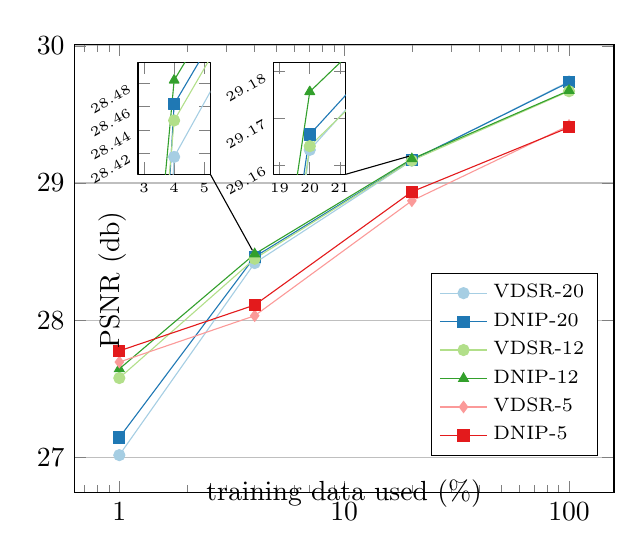
\begin{tikzpicture}
\begin{axis}[
    xmode=log,
    ymajorgrids,
    log ticks with fixed point,
                    % axis lines*=left,
    % for log axes, x filter operates on LOGS.
    % and log(x * 1000) = log(x) + log(1000):
    x filter/.code=\pgfmathparse{#1},
    x label style={at={(axis description cs:0.5,0.05)},anchor=north},
    y label style={at={(axis description cs:0.07,0.3)},anchor=west},
    xlabel={training data used (\%)},
    ylabel={PSNR (db)},
    legend style ={ at={(0.66,0.49)}, 
        anchor=north west, draw=black, 
        fill=white, align=left, font=\scriptsize},
    legend cell align={left},
    cycle list name={Paired-6},
    after end axis/.append code={\coordinate (a) at (axis description cs:0.33,0.54);},
    after end axis/.append code={\coordinate (c) at (axis description cs:0.62,0.75);}
    % cycle list name=black white
]
\addplot+[mark=*] table {
1 27.0168
4 28.4169
20 29.1632
100 29.7396
};
\addlegendentry{VDSR-20};

\addplot+[mark=square*]table{
1 27.1448
4 28.4622
20 29.1665
100 29.7342
};
\addlegendentry{DNIP-20};

\addplot+[mark=otimes*] table{
1 27.5787
4 28.4482
20 29.164
100 29.6691
};
\addlegendentry{VDSR-12};

\addplot+[mark=triangle*]table{
1 27.6454
4 28.4828
20 29.1757
100 29.6741
};
\addlegendentry{DNIP-12};

\addplot+[mark=diamond*] table{
1 27.6952
4 28.0328
20 28.8706
100 29.4195 
};
\addlegendentry{VDSR-5};

\addplot+[mark=square*] table{
1 27.7766
4 28.1107
20 28.9363
100 29.4053
};
\addlegendentry{DNIP-5};
% \begin{scope}[fill=white]
%     \spy[green!70!black,size=2.5cm] on (2.29,2.98) in node [right] at (0.2,4.4);
% \end{scope}
\end{axis}
\begin{scope}[xshift=23,yshift=115]
    \begin{axis}[
      xmin=3,xmax=5,
      ymin=28.41,ymax=28.49,
      y tick label style={rotate=30,anchor=east},
      line join=round,
      enlargelimits,
      width = 2.5cm,
      height = 3cm,
      tick label style={font=\tiny},
      cycle list name={Paired-6},
      after end axis/.append code={\coordinate (b) at (axis description cs:1,0);}
    ]
	\addplot+[mark=*]  coordinates {(1, 27.0168)
							(4, 28.4169)
							(20, 29.1632)
							(100, 29.7396)
							}; 
	\addplot+[mark=square*]coordinates{
							(1, 27.1448)
							(4 ,28.4622)
							(20 ,29.1665)
							};
	\addplot+[mark=otimes*] coordinates{
							(1 ,27.5787)
							(4 ,28.4482)
							(20 ,29.164)
							};
	\addplot+[mark=triangle*]coordinates{
							(1, 27.6454)
							(4, 28.4828)
							(20, 29.1757)
							};
	\end{axis}
	\draw[black] (a) -- (b);
\end{scope}

\begin{scope}[xshift=72,yshift=115]
    \begin{axis}[
      % xmode=log,
      xmin=19,xmax=21,
      ymin=29.16,ymax=29.18,
      y tick label style={rotate=30,anchor=east},
      line join=round,
      enlargelimits,
      width = 2.5cm,
      height = 3cm,
      tick label style={font=\tiny},
      cycle list name={Paired-6},
      after end axis/.append code={\coordinate (b) at (axis description cs:1,0);}
    ]
	\addplot+[mark=*]  coordinates {(1, 27.0168)
							(4, 28.4169)
							(20, 29.1632)
							(100, 29.7396)
							}; 
	\addplot+[mark=square*]coordinates{
							(1, 27.1448)
							(4 ,28.4622)
							(20 ,29.1665)
							(100, 29.7342)
							};
	\addplot+[mark=otimes*] coordinates{
							(1 ,27.5787)
							(4 ,28.4482)
							(20 ,29.164)
							(100, 29.6691)
							};
	\addplot+[mark=triangle*]coordinates{
							(1, 27.6454)
							(4, 28.4828)
							(20, 29.1757)
							(100, 29.6741)
							};
	\end{axis}
	\draw[black] (c) -- (b);
\end{scope}
\end{tikzpicture}

% \begin{tikzpicture}[y=.2cm, x=.7cm,font=\sffamily]
%  	%axis
% 	\draw (0,0) -- coordinate (x axis mid) (100,0);
%     	\draw (0,0) -- coordinate (y axis mid) (0,100);
%     	%ticks
%     	\foreach \x in {1,4,20,100}
%      		\draw (\x,1pt) -- (\x,-3pt)
% 			node[anchor=north] {\x};
%     	\foreach \y in {0,5,...,100}
%      		\draw (1pt,\y) -- (-3pt,\y) 
%      			node[anchor=east] {\y}; 
% 	%labels      
% 	\node[below=0.8cm] at (x axis mid) {Taining used (\%)};
% 	\node[rotate=90, above=0.8cm] at (y axis mid) {PSNR (db)};

% 	%plots
% 	\draw plot[mark=*, mark options={fill=white}] 
% 		file {div_soft.data};
% 	\draw plot[mark=triangle*, mark options={fill=white} ] 
% 		file {div_ciu.data};
% 	\draw plot[mark=square*, mark options={fill=white}]
% 		file {div_ciu_oscar.data};
% 	\draw plot[mark=square*]
% 		file {div_ciu_oscar_extrapolated.data};  
    
% 	%legend
% 	\begin{scope}[shift={(4,4)}] 
% 	\draw (0,0) -- 
% 		plot[mark=*, mark options={fill=white}] (0.25,0) -- (0.5,0) 
% 		node[right]{soft};
% 	\draw[yshift=\baselineskip] (0,0) -- 
% 		plot[mark=triangle*, mark options={fill=white}] (0.25,0) -- (0.5,0)
% 		node[right]{ciu};
% 	\draw[yshift=2\baselineskip] (0,0) -- 
% 		plot[mark=square*, mark options={fill=white}] (0.25,0) -- (0.5,0)
% 		node[right]{ciu + oscar};
% 	\draw[yshift=3\baselineskip] (0,0) -- 
% 		plot[mark=square*, mark options={fill=black}] (0.25,0) -- (0.5,0)
% 		node[right]{ciu + oscar extrapolated};
% 	\end{scope}
% \end{tikzpicture}
\end{document}